%!TEX root = ../../main.tex

\chapter{EDRICO (Educational DHBW RISC-V Core)}

The Proposed Processor design named EDRICO implements a basic RV32I
instruction set architecture. Besides the mandatory “Zicsr” extension no other
instruction set extensions are implemented. To keep the implementation simple and
straight-forward only one privilege mode (Machine-mode) is implemented. This mode
allows full access to the processor and peripherals. Future Versions could be
extended to implement S-Mode and U-Mode.\\
The core is a simple \acf{SISD} processor without any pipeline or even cache. The basic instruction cycle of fetch, decode, execute, store is performed for every instruction one at a time.\\
Figure \ref{fig:edricooverview} shows the full overview of the processor design:

\begin{figure}[H]
	\centering
	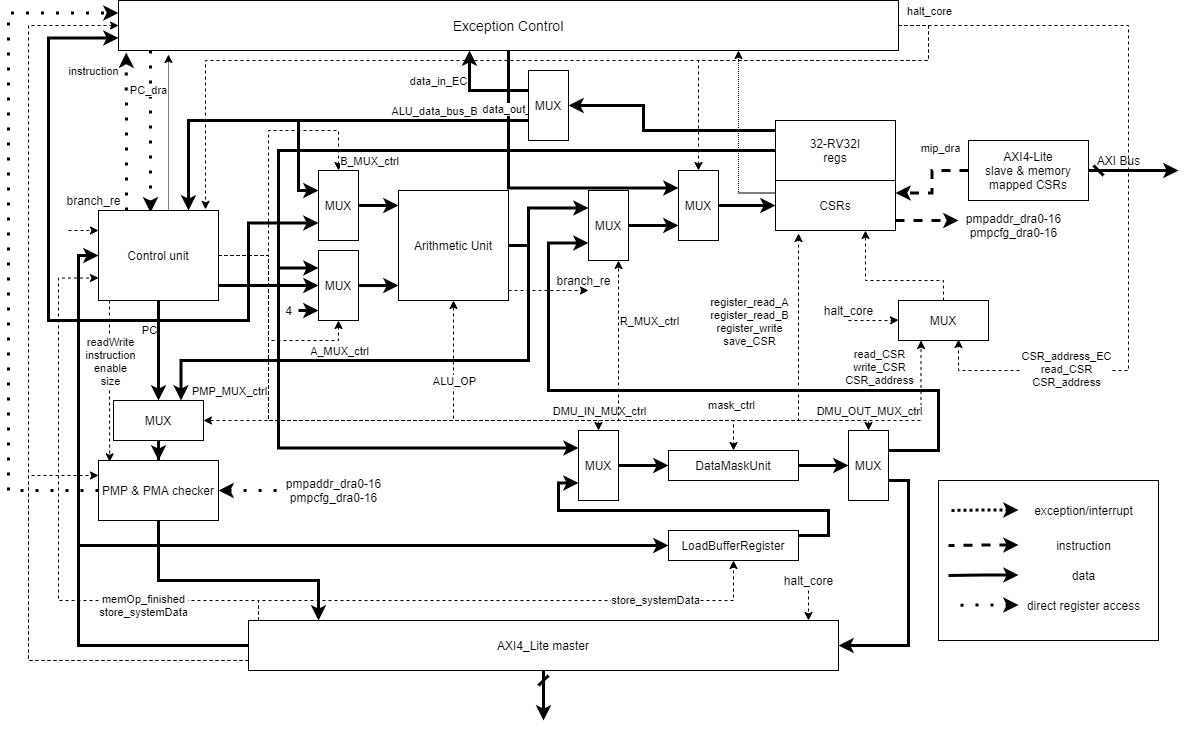
\includegraphics[width=150mm,scale=0.5]{datapath_EDRICO}
	\caption{EDRICO Overview}
	\label{fig:edricooverview}
\end{figure}

Its main components are the Exception Control, Control Unit, Arithmetic Unit,
Register Files, PMP \& PMA checker and the AXI4 Interfaces.
Each one of the components will be described in more detail in the following section.

\section{Control Unit}
The \ac{CU} is the heart of the processor and controls the other parts of the processor depending on the input instruction. The CU is responsible for fetching instructions from the instruction memory, decode the bitstream and set the respective control signals for the other processor components. Due to the complexity of the CU, there are several sub-modules which together form the overall CU.
\subsection{Architecture \& Design}
\label{CU_arch}
A general overview of the CU architecture is displayed in Figure \ref{fig:cuarchitecture}. 

\begin{figure}[H]
	\centering
	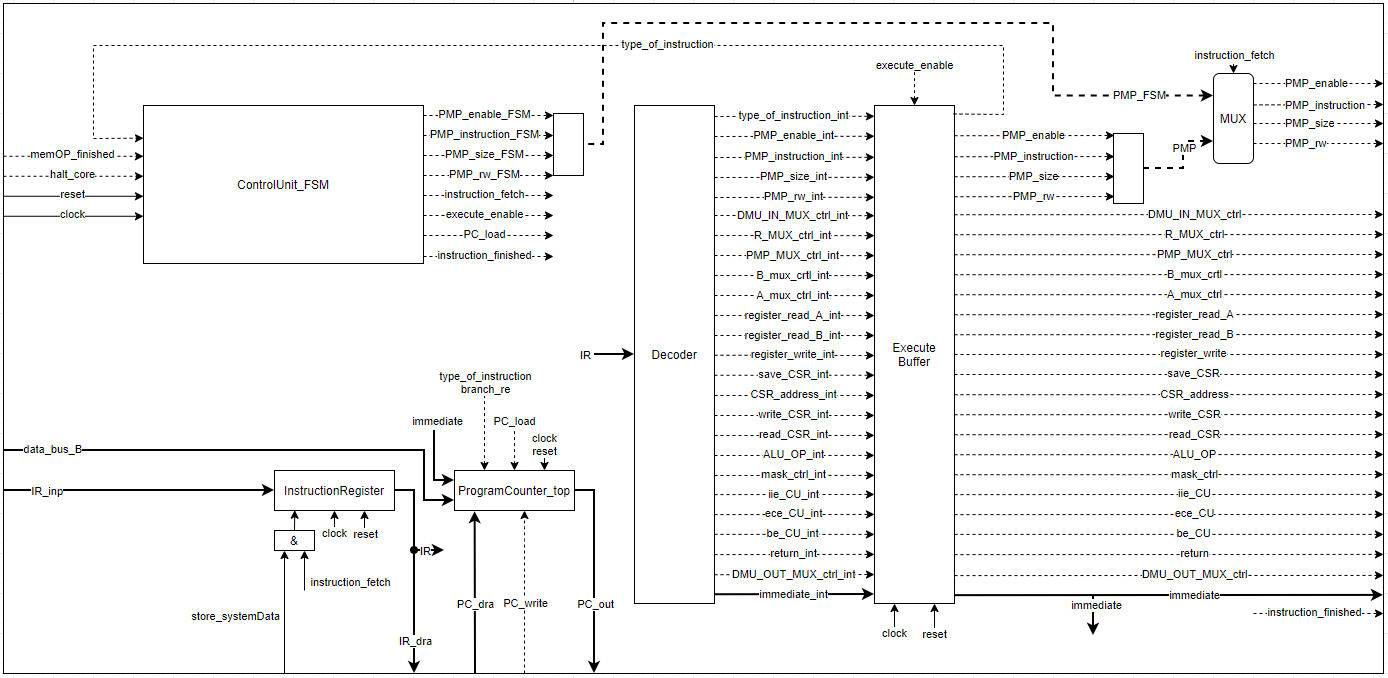
\includegraphics[width=\textwidth]{CU_architecture}
	\caption{Control Unit Architecture}
	\label{fig:cuarchitecture}
\end{figure}

To describe the functionality of the CU in more detail, every sub-module will be described closely.\\
Since the Control Unit is responsible for the whole processor, it is important to have a persistent and stable procedure for every instruction that shall be executed. The Control Unit \ac{FSM} is responsible for the correct clock timings which is important due to memory operations and the execution time of the other processor parts. The states and conditions of the FSM are displayed in Figure \ref{fig:cufsm}. 

\begin{figure}[H]
	\centering
	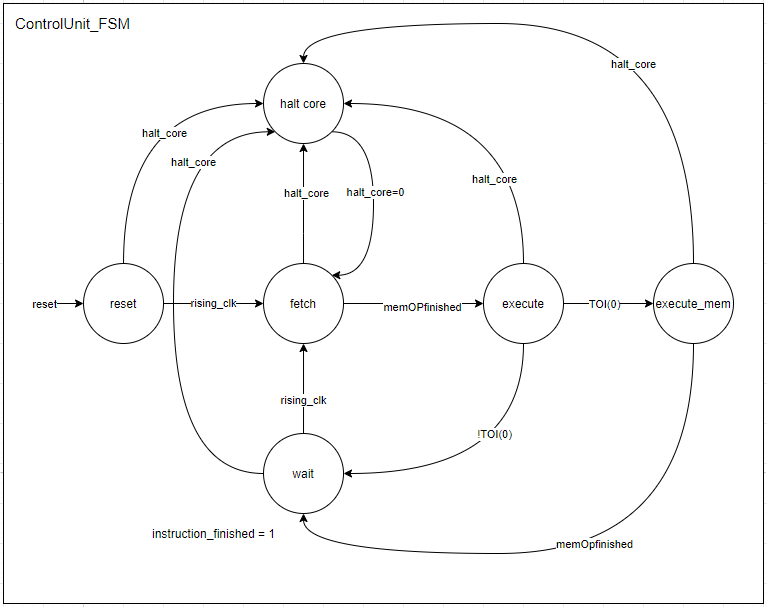
\includegraphics[width=\textwidth]{CU_FSM}
	\caption{Control Unit FSM overview}
	\label{fig:cufsm}
\end{figure}

Table \ref{tableFSM} shows a more detailed overview of the clock cycles and the corresponding actions and states:\\

\begin{table}[h]
\resizebox{\textwidth}{!}{
	\begin{tabular}{|c|c|l|l|}
		\hline
		\textbf{ClockCycle} & \textbf{Edge} & \textbf{Action} & \textbf{Signal} \\
		\hline
		1 & rising & pass the PC and enable PMP \& PMA checker with respective information &  \\
		\hline
		& falling & N/A &  \\
		\hline
		4 & rising & data is ready in instruction register - switch to execute state & \textit{memOPfinished} \& \textit{store\_systemData} is high \\
		\hline
		5 & rising & execution is started - if memory operation wait for another \textit{memOPfinished} flag, otherwise wait & \textit{execute\_enable} \\
		\hline
		x & rising & during memory operation: data loaded to buffer \textbackslash store transfer finished $\rightarrow$ wait state & \textit{memOPfinished} \& \textit{store\_systemData} is high \\
		\hline
		& falling & if load: store data form buffer to specified location &  \\
		\hline
		6 / x+1 & rising & go to \textit{fetch\_state} &  \\
		\hline
	\end{tabular}}
\caption{Timing of FSM}
\label{tableFSM}
\end{table}

During an execution cycle, the FSM controls the rest of the CU consisting of memory, decoding unit, PC control and the different multiplexers. To understand what the purpose of the different signals are, the other components of the Control Unit are described in the following sections.

After loading an instruction from the memory to the instruction register, the decoding process can begin. The responsible part for this process is the decoding unit which is described below.(Also visible in figure \ref{fig:cuarchitecture})\\
In this project the RISC-V RS32I instruction set is used which consists of 32-bit instruction words. The instruction words have a pre-defined structure and are divided into six instruction formats.
The instruction formats are shown in Figure \ref{fig:instrtypes}.

\begin{figure}[h]
	\centering
	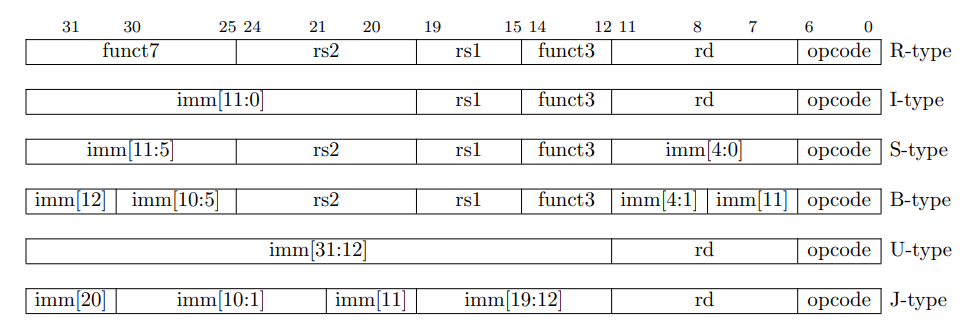
\includegraphics[width=\textwidth]{instr_types.png}
	\caption{RISC-V Instruction formats \cite{riscv}}
	\label{fig:instrtypes}
\end{figure}
The different instruction formats are useful for the decoding process since e.g. all LOAD instructions have the same structure and therefore, the effort to decode the 32-bit word can be reduced. Since the control signals are unique for every instruction and depending on the content of the 32-bit word, the decoder has to identify the encoded instruction, extract the information and respectively set the control signals, calculate immediates and control the multiplexers. A more detailed description of the decoding process can be found in section \ref{CU_impl}.\\
After the instruction is decoded, all output control signals are stable and ready to be fed through. Before leaving the CU, the \textit{Execute Buffer} (figure \ref{fig:cuarchitecture}) buffers the control signals. Once the FSM sets the \textit{execute\_enable} flag, the control signals are fed through. This buffer prevents the processor to confuse timing and clock cycles, or use signals which are not yet set correctly.\\
During an instruction execution, the program counter has to be incremented for the processor to know what instruction will follow. \textit{But} since there are several instructions that modify the program counter, a so called \textit{PC control} is designed. The PC control receives information from the decoder which consists of a 4 bit signal. The different instructions and the respective action as well as the respective control signal are shown in following table \ref{PCcontrol}:\clearpage

\begin{table}[h]
	\resizebox{\textwidth}{!}{
		\begin{tabular}{|l|l|l|}
			\hline
			\textbf{Instruction} & \textbf{Action} & \textbf{Control Signal}\\
			\hline
			Default & No action required & \textbf{0000}\\
			\hline
			Branch & Depending on the result of branch operation, PC will be incremented respectively & \textbf{0010}\\
			\hline
			JAL & Target address obtained by adding current PC and immediate, rejump address stored in register & \textbf{0100}\\
			\hline
			JALR & Target address obtained by adding input register to immediate & \textbf{1000}\\
			\hline
		\end{tabular}}
	\label{PCcontrol}
	\caption{Program Counter control: Instructions and resulting actions}
\end{table}
For instructions which do not influence the program counter, the standard operation performs the \textbf{PC + 4} operation.

The instruction register displayed in figure \ref{fig:cuarchitecture} manages the instruction string coming from the memory.
All of these parts together form the Control Unit and are responsible for the correct execution of the instructions. The implementation of the sub-units in VHDL are described in the following section \ref{CU_impl}.\clearpage

\subsection{Implementation}
\label{CU_impl}
The implementation of the Control Unit is split up into multiple sub-implementations. As shown in figure \ref{fig:cuarchitecture} those sub-modules are the \textit{FSM, decoder, execute\_buffer, PC control and instruction register}. Since the implementation of the FSM is very similar to other FSM implementations in this project, the detailed description of a FSM in VHDL is found in the next chapters.\\
In this section the implementation of the decoder will be described more closely.
As already described in section \ref{CU_arch} the instructions can be separated in different instruction formats. To distinguish the different instructions, so-called \textit{instruction clusters} are created. These clusters sum up instructions which are encoded in the same instruction format or in general are similar.
The following table shows the different clusters and the corresponding instructions:
\begin{table}[h]
	\centering
		\begin{tabular}{|l|l|}
			\hline
			\textbf{Cluster} & \textbf{Instructions}\\
		
			\hline
			LOAD & Load - Byte \textbackslash Halfword \textbackslash Word\\
			
			\hline
			STORE & Store - Byte \textbackslash Halfword \textbackslash Word\\
			
			\hline
			BRANCH & Different Branch Instructions (e.b. Branch if equal)\\
			
			\hline
			JALR & only JALR, since it has a unique instruction structure\\
			
			\hline
			JAL & only JAL, since it has a unique instruction structure\\
			
			\hline
			OP & All arithmetic instructions like ADD, SUB, shift and comparisons\\
			
			\hline
			OP-IMM & All arithmetic instructions performed with immediate\\
			\hline
			AUIPC & only AUIPC, since it has a unique instruction structure\\
			\hline
			LUI & only LUI, since it has a unique instruction structure\\
			\hline			
	\end{tabular}
	\label{instructioncluster}
	\caption{Decoding instruction clusters}
\end{table}


To determine the cluster for each instruction, a decoding procedure is implemented in VHDL based on structure visualized in figure \ref{fig:decode_structure}:

\begin{figure}[H]
	\centering
	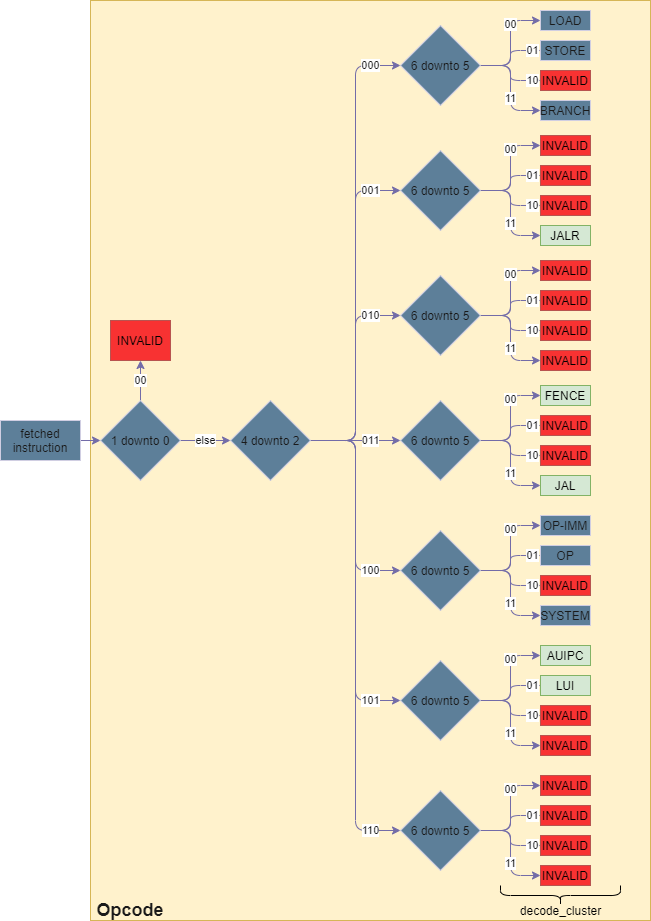
\includegraphics[width = 120mm]{Decode_Structure}
	\caption{Decoding Structure to determine instruction cluster}
	\label{fig:decode_structure}
\end{figure}
After determining the cluster, the VHDL code assigns all the outputs visible in figure \ref{fig:cuarchitecture} with the respective information. For a better understanding of the information extraction, figure \ref{fig:instruction_bits} shows how the 32-bit instruction word is split up (in this case for the \textit{OP} and \textit{OP-IMM} instructions.)
\begin{figure}[H]
	\centering
	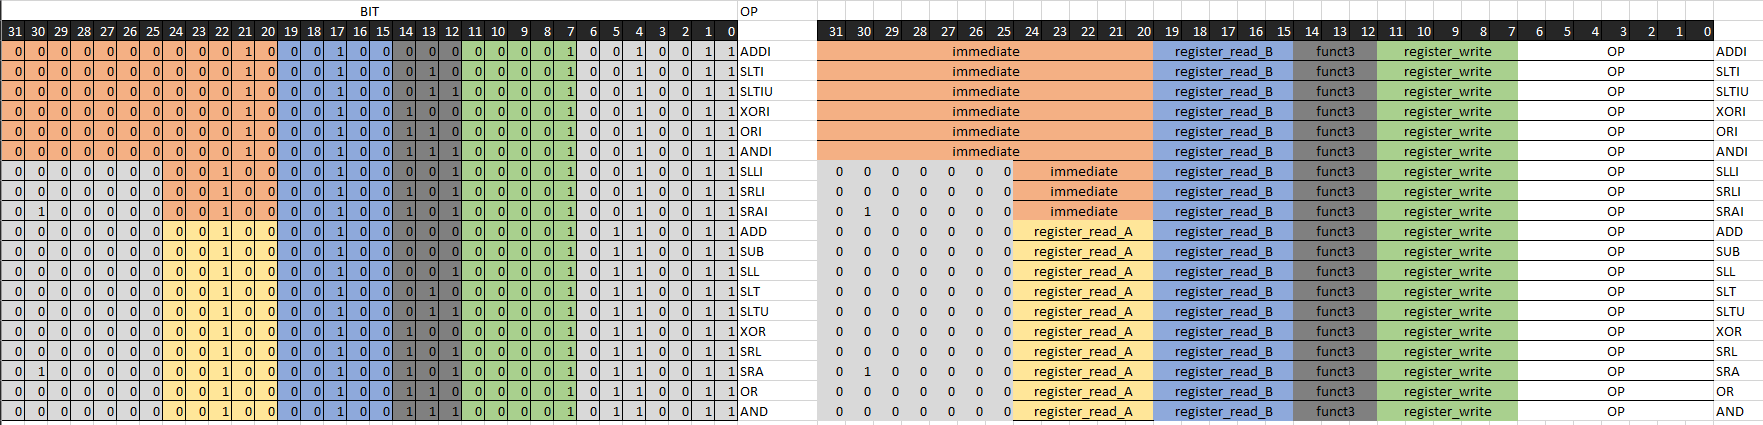
\includegraphics[width = 200mm,angle = 270, origin = c]{instruction_bits}
	\caption{Information extraction from 32-bit instruction word}
	\label{fig:instruction_bits}
\end{figure}


\section{Arithmetic Logical Unit}
The \acf{ALU} is the part of the processor that performs the arithmetic and logical operations. Figure \ref{fig:alu} gives an overview of what type of operations are performed.
\begin{figure}[H]
	\centering
	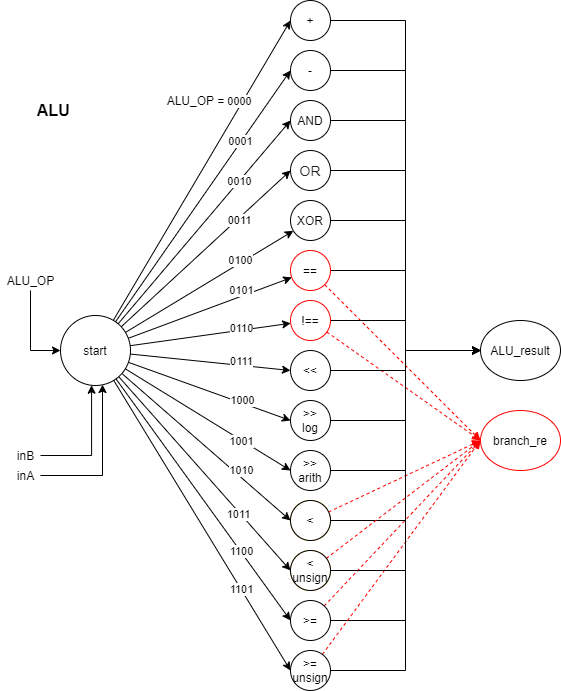
\includegraphics[width=\textwidth]{ALU.png}
	\caption{ALU operations}
	\label{fig:alu}
\end{figure}

\subsection{Architecture \& Design}
To implement the ALU, it is required to have the data inputs as well as clock input and a control signal consisting of 4 bits to specify the required operation to be performed. Since there are instructions that require a branch response to know whether the next instructions shall be skipped or not, the ALU needs an additional output called \textit{branch\_re} other than the result output of the arithmetic/logical operation. The architecture of the ALU is shown in figure \ref{fig:alu_arch}:
\begin{figure}[H]
	\centering
	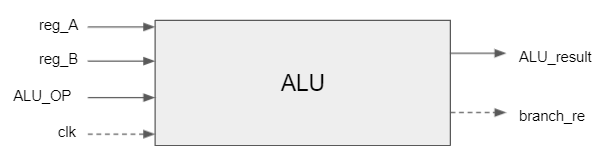
\includegraphics[width=\textwidth]{alu_arch.png}
	\caption{ALU operations}
	\label{fig:alu_arch}
\end{figure}
Not only the instructions e.g. \textit{ADD, SUB, XOR...} require an arithmetic operation but also \textit{LOAD, STORE..} require an ALU action. While \textit{ADD, SUB, XOR...} require an operation between the two input values (either register-register or register-immediate) to get a mathematical or logical result, the \textit{LOAD, STORE...} instructions require the ALU to build the target addresses for the memory access.
\subsection{Implementation}
The implementation of the ALU is based on figure \ref{fig:alu} and performs a switch-case on all the different input values of \textit{ALU\_OP}. The 4-bit input variable specifies the operation based on following declarations:
\begin{table}[H]
\centering
	\begin{tabular}{|c|c|}
		\hline
		\textbf{ALU\_OP} & \textbf{Operation} \\
		\hline
		0000 & ADD \\
		\hline
		0001 & SUB \\
		\hline
		0010 & AND \\
		\hline
		0011 & OR \\
		\hline
		0100 & XOR \\
		\hline
		0101 & EQUAL \\
		\hline
		0110 & NEQUAL \\
		\hline
		0111 & shift\_left \\
		\hline
		1000 & shift\_right \\
		\hline
		1001 & shift\_right (arithmetic) \\
		\hline
		1010 & <\\
		\hline
		1011 & < (unsigned) \\
		\hline
		1100 & $\geq$ \\
		\hline
		1101 & $\geq$ (unsigned) \\
		\hline
	\end{tabular}
\caption{Input code and respective operation}
\end{table}
To visualize the implementation, a part of the VHDL code is displayed in the following. The case statement is based on the input \textit{alu\_op}. The ALU then performs the corresponding operation with the two inputs \textit{in\_a and in\_b}.\clearpage

\begin{lstlisting}[style=vhdl, caption=ALU VHDL code]
begin
	process(in_a, in_b, alu_op)
	begin
	--default output is 0
	branch_re <= '0';
	alu_result <= "00000000000000000000000000000000";	
		case alu_op is	
			when "0000" =>--"ADD"	
				alu_result <= in_b + in_a;	
			when "0001" =>--"SUB"	
				alu_result <= in_b -in_a;	
			when "0010" =>--"AND"	
				alu_result <= in_b AND in_a;
			when "0011" =>--"OR"
				alu_result <= in_b OR in_a;
			when "0100" =>--"XOR"
				alu_result <= in_b XOR in_a;
			when "0101" =>--"EQUAL"	
				if(in_b = in_a) then
				branch_re <= '1';
				else
				branch_re <= '0';
				end if;
	...
\end{lstlisting}
In case the operation determined by \textit{alu\_op} might be originating of a branch instruction, the \textit{branch\_re} flag has to be set respectively (line  19). Since the branch instructions only include some of the arithmetic and logical operations of the ALU, the default value for the \textit{branch\_re} is set as \textit{0}.

\section{\acf{RF}}
The Register can be used to store data and configure the core. General Purpose
registers are mostly used to temporarily store data like operands and results of
calculations. The CSR Register File is used to configure the core and retrieve
information about it. More detailed information about these two RFs can be found in
the following chapters.
\clearpage
\subsection{Architecture \& Design}
The architecture of the register files is shown in following figure \ref{fig:RF_arch}

\begin{figure}[H]
	\centering
	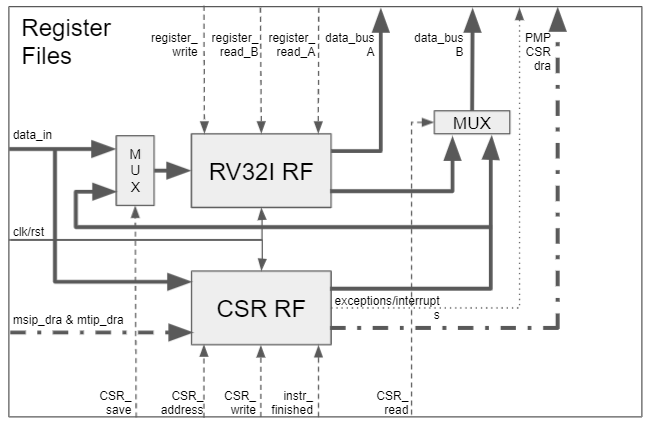
\includegraphics[width=\textwidth]{RF_arch.png}
	\caption{Register Files architecture}
	\label{fig:RF_arch}
\end{figure}

In order to write data to a register, the value needs to be put on the \textit{data\_in} bus and the corresponding control signals need to be configured. Data can be read either via the \textit{data\_busA} or \textit{data\_busB}, the CSR registers can only be accessed on \textit{data\_busB} via a MUX controlled by the \textit{CSR\_read} signal. If the bit is set, the CSR specified by \textit{CSR\_address} will be visible on \textit{data\_busB} at the next rising clock edge.\\
In order to store data to a CSR register, it has to be put on the \textit{data\_in} bus. If the \textit{CSR\_write} bit is set, the data is saved to the register specified by \textit{CSR\_address} on the next falling clock edge.\\
If the \textit{CSR\_save} signal is applied, the CSR Register File output is connected to the data input bus of the general purpose registers. This allows to save CSR data directly to the RV32I registers without using the system data bus. Some of the CSR registers allow direct memory accesses, e.g. the \textit{msip\_dra} \& \textit{mtip\_dra} signals are used to set the software and timer interrupt pending bits respectively. To increase the performance of memory accesses, the PMP CSRs can be read via a dedicated bus.\\
While the CSR RF is accessed by 12 Bit addresses, RV32I registers are accessed without addressing in order to decrease decoding time. Therefore, each register requires three Signals resulting in a total of 96 signals for read and write. The RFs are clocked with the system clock and reset on system reset. As per usual, data is stored on the falling clock and displayed on the rising clock.

\subsection{Implementation}

\section{PMP \& PMA Checker}
\subsection{Architecture \& Design}
\subsection{Implementation}

\section{Exception Control}
\subsection{Architecture \& Design}
\subsection{Implementation}

\section{AXI4-Lite Master}
\subsection{Architecture \& Design}
\subsection{Implementation}

\section{AXI4-Lite Slave}
\subsection{Architecture \& Design}
\subsection{Implementation}
